\documentclass[3p,12pt]{elsarticle}

\usepackage{amssymb}
\usepackage{hyperref}
\usepackage{rotating}
\usepackage{multirow}
\usepackage{tabularx}
\usepackage{comment}
\usepackage{array}

\journal{TBD}

%% DOCUMENT %%
\begin{document}

%% 
\begin{frontmatter}

\title{A Systematic Literature Review on Extensions to Role Based Access Control}

\author{Eric D. Helms, JeeHyun Hwang, Tao Xie, Laurie Williams}
\address{North Carolina State University}
\address{Department of Computer Science}
\address{890 Oval Drive, Box 8206}
\address{Raleigh, NC 27695-2858}


\begin{abstract}

\noindent
{\bf Context}: Since the introduction of the role based access control (RBAC) standard in the late 1990's, 
RBAC has become an increasingly popular access control mechanism for applications such as 
web applications, mobile computing and databases. RBAC restricts access to resources 
based on the identity of subjects connected to logical groupings of permissions.  
The introduction of computing into new domains has led to proposals for extensions to the standard
RBAC model; for example, defining additional constraints among roles, adding context or defining new heirarchy relationships.
\\
\\
\noindent
{\bf Aim}: Our work aims to aid researchers looking to expand on the body of knowledge surrounding extensions to RBAC need a starting place to prevent re-invention of the wheel and
developers needing to find and select an access control mode based on their project requirements. 
\textit{The goal of this work is to provide practioners an assessment of the current extensions to RBAC to aid with choosing a model that meets their requirements, and researchers with insights into the state of RBAC extension models and how they are evaluated.}
\\
\\
\noindent
{\bf Method}: We conducted a systematic literature review by collecting and synthesizing relevant research
papers in the area of RBAC extensions. The review we performed yielded 1716 papers, of which 29 were deemed primary sources 
for inclusion as model extensions to the RBAC standard model. The papers we collected were from electronic digital libraries
IEEE, Google Scholar, CiteSeerX and ACM based on a set of exclusion and inclusion criteria.  
We performed a comparative analysis of the primary sources to find relationships among extended models and to analyze the state of RBAC extension evaluations.
\\
\\
\noindent
{\bf Results}: Our results showed that extensions to RBAC fall into a number of categories that in turn all
fall under the single category of context based extensions.  We look into the motivations behind RBAC extensions and
the domains that are leading factors in developing these newer models. We also quantify the current evaluation methods
used when RBAC extension models are presented to the research community.
\\
\\
\noindent
{\bf Conclusions}: The extensions to RBAC fall into a number of categorizations with Organization, Privacy, Resource, Task, Spatio-Temporal, Spatial and Temporal falling under the general category of context.
Domains, such as healthcare and mobile computing, were idenitfied as motivations behind the development of extensions to the RBAC model.  Our literature review showed that the state of RBAC model evaluation could benefit from the research community given most model evaluations seen within the papers were based on hypothetical situations with little to no case studies or implementations in practice.

\end{abstract}


\begin{keyword}
%% keywords here, in the form: keyword \sep keyword
RBAC \sep access control \sep systematic literature review
\end{keyword}

\end{frontmatter}


%% SECTIONS %%
\section{Introduction} \label{sec:introduction}

Why is the base model of RBAC extended by newer models?

P1: Note history of the RBAC model, statistics, and official status

P2: Mention extensions exist in response to developments and new domains over time

P3: Mention audience, why they should care, and why exploring extensions space is important in relation to the reason the standard was originally concieved

P4: Talk about what this work is going to do, goal, brief process

P5: List goals or contributions

P6: Outline paper and sections


Role based access control (RBAC) was first introduced in the 1990 when the National Instittute for Standards and Technology (NIST) requested that a unified standard be created.  proposed standard RBAC model \cite{ferraiolo}

Role-based access control (RBAC) models \cite{ferraiolo} became popular used to govern access to critical resources.  In an RBAC model, roles represent a group of users who are involved in a specific job function in an organization. RBAC assigns permissions of specific actions on resources to roles instead of individual users.  Therefore, in order to gain roles' permission on specific resources, users acquire appropriate roles first.

RBAC is a generalized access control approach used for various applications including web services, database applications, and healthcare applications.  RBAC has advantages in maintaining and managing organization's security policies.  For example, if a user is to access manager role's resources within a given organization, security policy administrators simply add the user to be associated with the manager role.

Standard RBAC model considers only role-user association and role hierarchy.
Since standard RBAC model has limitations such as specifying environmental constraints or context information
Researchers developed extended models of RBAC to overcome the limitations.
However, as researchers often develop their own specialized extended models of RBAC,
their research cannot be generalized or compared with other research work appropriately.
As a result, researchers could take time on reinventing the wheel.
But how do we, as a community, ensure that a metric is suitable and acceptable for its intended purpose?

The goal of this work is to synthesize available research results on extended models of RBAC. We analyze their extended features and claimed research contributions to find limitations of current RBAC models and what extent of extended features by
comparing with similar research work.
We conducted a systematic literature review (SLR) to evaluate and interpret all available research relevant to a particular research question or topic area of interest.

Our research give benefits to a community as follows:

\begin{itemize}
\item Our work summarizes current extended RBAC research work and its contributions. By synthesizing the current results, our work shows a roadmap of current extended RBAC research.
\item Our work guides a direction for a standard of extended RBAC. Understanding the categorization and the motivation of the existing research results helps decide a standard of extended RBAC.
\item Our work shows a criteria in comparison among research results.
\item Our work helps identify the research challenges in the ares of security policies and suggest a future extension of RBAC.
\end{itemize}

\section{Core Role Based Access Control} \label{sec:core-rbac}

Since the basis for our review is extensions to the core model, we will describe the core model, associated entities and other terminology encountered across the space of our review.  The NIST RBAC model proposed by Ferraiolo et al. and later adopted as the official standard for RBAC by the International Committee for Information Technology Standards (INCITS) consists of four basic entities:

\begin{itemize}
\item a set of users \emph{Users}: A user can be a person or an agent.
\item  a set of roles \emph{Roles}: A role is a collection of permissions to perform a specific job function in an organization.
\item a set of permissions \emph{Permissions}: A permission refers to an access mode that can be exercised on an object in the system and a session relates a user to possibly many roles.
\item a set of sessions \emph{Sessions}: In each session, a user can be assigned to some of the roles, only when the corresponding role is enabled for activation for that time.		
\end{itemize}

In the RBAC, a user can exercise a permission only if the user are assigned to a role.
In addition to the four basic components, two functions are defined:
the user role assignment (UA) and the role
permission assignment (PA) functions.
UA models assignment of users to roles.
PA models assignment of permissions to roles.

%Each user incorporates a session    
%The user function maps each session to a
%single user, whereas the role function establishes a
%mapping between a session and a set of roles activated
%by the corresponding user in the session.

P1: Describe RBAC entities

P2: Note the 4 levels of RBAC

P3: Concisely describe level 1

P4: Concisely describe level 2

P5: COncisely describe level 3

P6: Concisely describe level 4


\section{Methodology and Process} \label{sec:process}

The systematic literature review process was developed ahead of time and agreed upon by the researchers following recommendations from Kitchenham's suggested processes \cite{kitchenham2007guidelines}.  The systematic literature review was performed in four stages:

\begin{itemize}
\item Development of a search strategy
\item Elimination of papers based on title
\item Elimination of papers based on abstract
\item Elimination of papers based on content and matching to elimination criteria
\end{itemize}

\subsection{Search Strategy}

For the first phase of our systematic literature review, an automated comprehensive search of multiple academic search engines was performed. The list of search engines were:

\begin{itemize}
\item Google Scholar - \url{http://scholar.google.com}
\item IEEExplore - \url{http://ieeexplore.ieee.org}
\item ACM Portal - \url{http://dl.acm.org}
\item CiteSeerX - \url{http://http://citeseerx.ist.psu.edu/index}
\end{itemize}

For each of the criteria below, a search was performed on each of the search engines for a total of 12 data sets.  The criteria used were:
\begin{itemize}
\item role based access control
\item RBAC
\item role-based access control
\end{itemize}

The search performed was done in an automated way using a set of scripts to query and collect data from each search engine with the criteria string as input.  For each criteria for each search engine, the results were captured until a stopping criteria was met.  Each run was performed as follows:

\begin{enumerate}
\item Remote call to search engine with current search start position and the current search criteria.
\item Parse results and extract paper title, authors and year of publication.
\item Compare results against stopping criteria.
\end{enumerate}

\begin{itemize}
\item If stopping criteria met, stop search.
\item If stopping criteria not met, increase search position by number of results and return to step 1.
\end{itemize}

The stopping criteria used was either after the first 1000 results, a limitation imposed by some of the search engines, or if ten consecutive results did not contain the search criteria phrase within the title.  After gathering all 12 data sets, the data was combined into a master list by systematically comparing the bibliographic information for each.  After producing a master list, a series of assessment rounds were performed to narrow the paper list and identify primary sources.

\subsection{Elimination Rounds}

The elimination rounds were performed based on reading of the title, abstract and finally the paper itself.  While each elimination stage had a unique set of criteria for elimination the general procedure for elimination for the researchers was as follows.

\begin{itemize}
\item Each reviewer independently classified papers as relevant, irrelevant or uncertain.
\item Those papers marked as relevant by both reviewers were kept and those marked irrelevant by both were thrown out.
\item Papers marked as relevant, or irrelevant by a single reviewer were combined with all papers marked as uncertain and discussed by both reviewers.  From this discussion, papers were either thrown out or kept until the next round of the review.  Ties were broken by an indepedent party.
\end{itemize}

The title elimination round was based off of whether role based access control and model were mentioned directly.

The second round of elimination was based off on reading the abstracts of the remaining papers.  The inclusion criteria for the abstract reading tried to answer the following questions:

\begin{itemize}
\item Does the abstract mention a proposed model?
\item Does the abstract mention extension of role-based access control?
\item Does the abstract mention either an implementation, evaluation or domain for their model?
\end{itemize}

The results of the searches is summarised below:

\begin{tabular}{|l|l|l|l|l|}
\hline
\textbf{Search Engines} & 
\textbf{RBAC} & 
\textbf{role based access control} & 
\textbf{role-based access control} & 
\textbf{Total}
\\\hline

Google Scholar & 651 & 213 & 435 & 1299
\\\hline
ACM Portal & 500 & 20 & 720 & 1240
\\\hline
IEEExplore & 200 & 40 & 230 & 470
\\\hline
CiteSeerX & 100 & 100 & 150 & 350
\\\hline
 &  &  &  & 
\\\hline
Totals & 1451 & 373 & 1535 & 3359
\\\hline

Combined &  &  &  & \textbf{1716}
\\\hline
\end{tabular}

\section{RQ1: Classification} \label{sec:categorization}

\textit{How can RBAC extension models be classified?}
\\

During the paper reading phase, we identified that a variety of common terms were emerging to describe the RBAC extension models. 
We developed a process by which to build a classification of the RBAC extension models based upon observations during the paper reading phase.
For example, the paper ``Privacy-aware role-based access control'' \cite{ni2010privacy} brings in the notion of privacy explicitly within the title of the paper and the name of their model. 
Some papers appeared to present a direct pronouncement of their classification, whereas others were less obvious.
Thus, we developed a set of guidelines to aide in determining a set of eight categories. 
In developing these guidelines, we defined each category by a single noun-phrase descriptor.
The guidelines were as follows:

\begin{itemize}
\item Model Name - Does the name of the model classify itself?
\item Self Assessment - Do the authors of the paper directly identify a descriptor for their model within the body of the paper?
\item Repetition of Phrase - Does the body of the paper present the same phrase repeatedly when discussing their model?
\end{itemize}

The previous example paper ``Privacy-aware role-based access control'' \cite{ni2010privacy} contained ``privacy'' in the title and in the name of the model leading to the creation of the Privacy category and the subsequent placement of the paper under that category.
By comparison, the paper ``An extended RBAC model based on granular logic'' \cite{jian2008extended} does not contain a direct categorization in the title or model name. 
However, in reading the body of the paper, we determined that the paper discussed RBAC extension based on context. 
In Section 4.1, we offer definitions for each of the eight observed categories.

\subsection{Results}

We provide a definition for each observed model category based on data extracted from the primary sources and the English definitions for each noun-phrase.
Some category descriptors contain abbreviations in parenthesis that match the shortened name found in Table 6 (within Appendix 1) which presents each primary source within it's designated category.

\begin{itemize}

  \item \textbf{Context}: The extension model integrates contextual information into the RBAC standard model. Context is defined as a user's current state and environment (e.g., location, time, system resources, network state, network security configuration, etc). The user's access privileges are dependent upon the values of the current state and environment at any given time.

  \item \textbf{Constraint (Const)}: The extension model provides conditional restrictions on permissions of given roles. The constraint is either static or dynamic. For example, a doctor may modify any medical record for which the doctor is assigned as the designated primary care physician. This example describes a doctor's permission with a conditional restriction - ``only when the doctor is assigned as the designated primary care physician may the doctor modify a particular medical record''.

  \item \textbf{Organizational (Org)}: The extension model is concerned with providing mechanisms and entities that allow for RBAC across multiple organizations. Typically, users may have the same role name in different organizations, but may have different access privileges due to departmental variations.
  
  \item \textbf{Privacy (Priv)}: The extension model provides entities and mechanisms to describe privacy policies, which are legal statements or documents about disclosure or management of personally identifiable information such as name, address, or date of birth.
  
  \item \textbf{Task}: The extension model provides task entities which are associated with permissions and roles. A task is a fundamental unit of a business activity. Different from core RBAC, in task-role-based access control model, roles are not directly associated with permissions. Roles are associated with tasks that are associated with permissions. For example, the employee role is associated with a task to write a report. This task is then associated with a permission.

  \item \textbf{Spatio-Temporal}: The extension model combines the use of either or both spatial (location-based) and temporal (time-based) constraints in specifying access control policies. For example, specific locations permit roles to conduct actions from 8:00 a.m. to 5:00 p.m.

  \item \textbf{Spatial}: The extension model provides spatial (location-based) constraints in specifying access
	control policies. For example, in organizations, locations are enforced whereas a
	specific role is permitted to conduct an action. Consider that an employee works only at a specific location.
	In such cases, a role should allow access to required resources only when the user is in that location. 
	Spatial constraints can integrate with roles, user-role assignments, or role-permission assignments. 

  \item \textbf{Temporal (Temp)}:  The extension model provides temporal (time-based) constraints in specifying access
	control policies. For example, in organizations, periodic temporal durations are enforced whereas a
	specific role is permitted to conduct an action. Consider that a temporal employee works only from 9:00 a.m. to 3:00 p.m.
	In such cases, the temporal employee role should only be allowed to access required resources during the interval. 
	Temporal constraints can integrate with roles, user-role assignments, or role-permission assignments.   
	
\end{itemize}

\begin{figure}[ht]
    \centering
        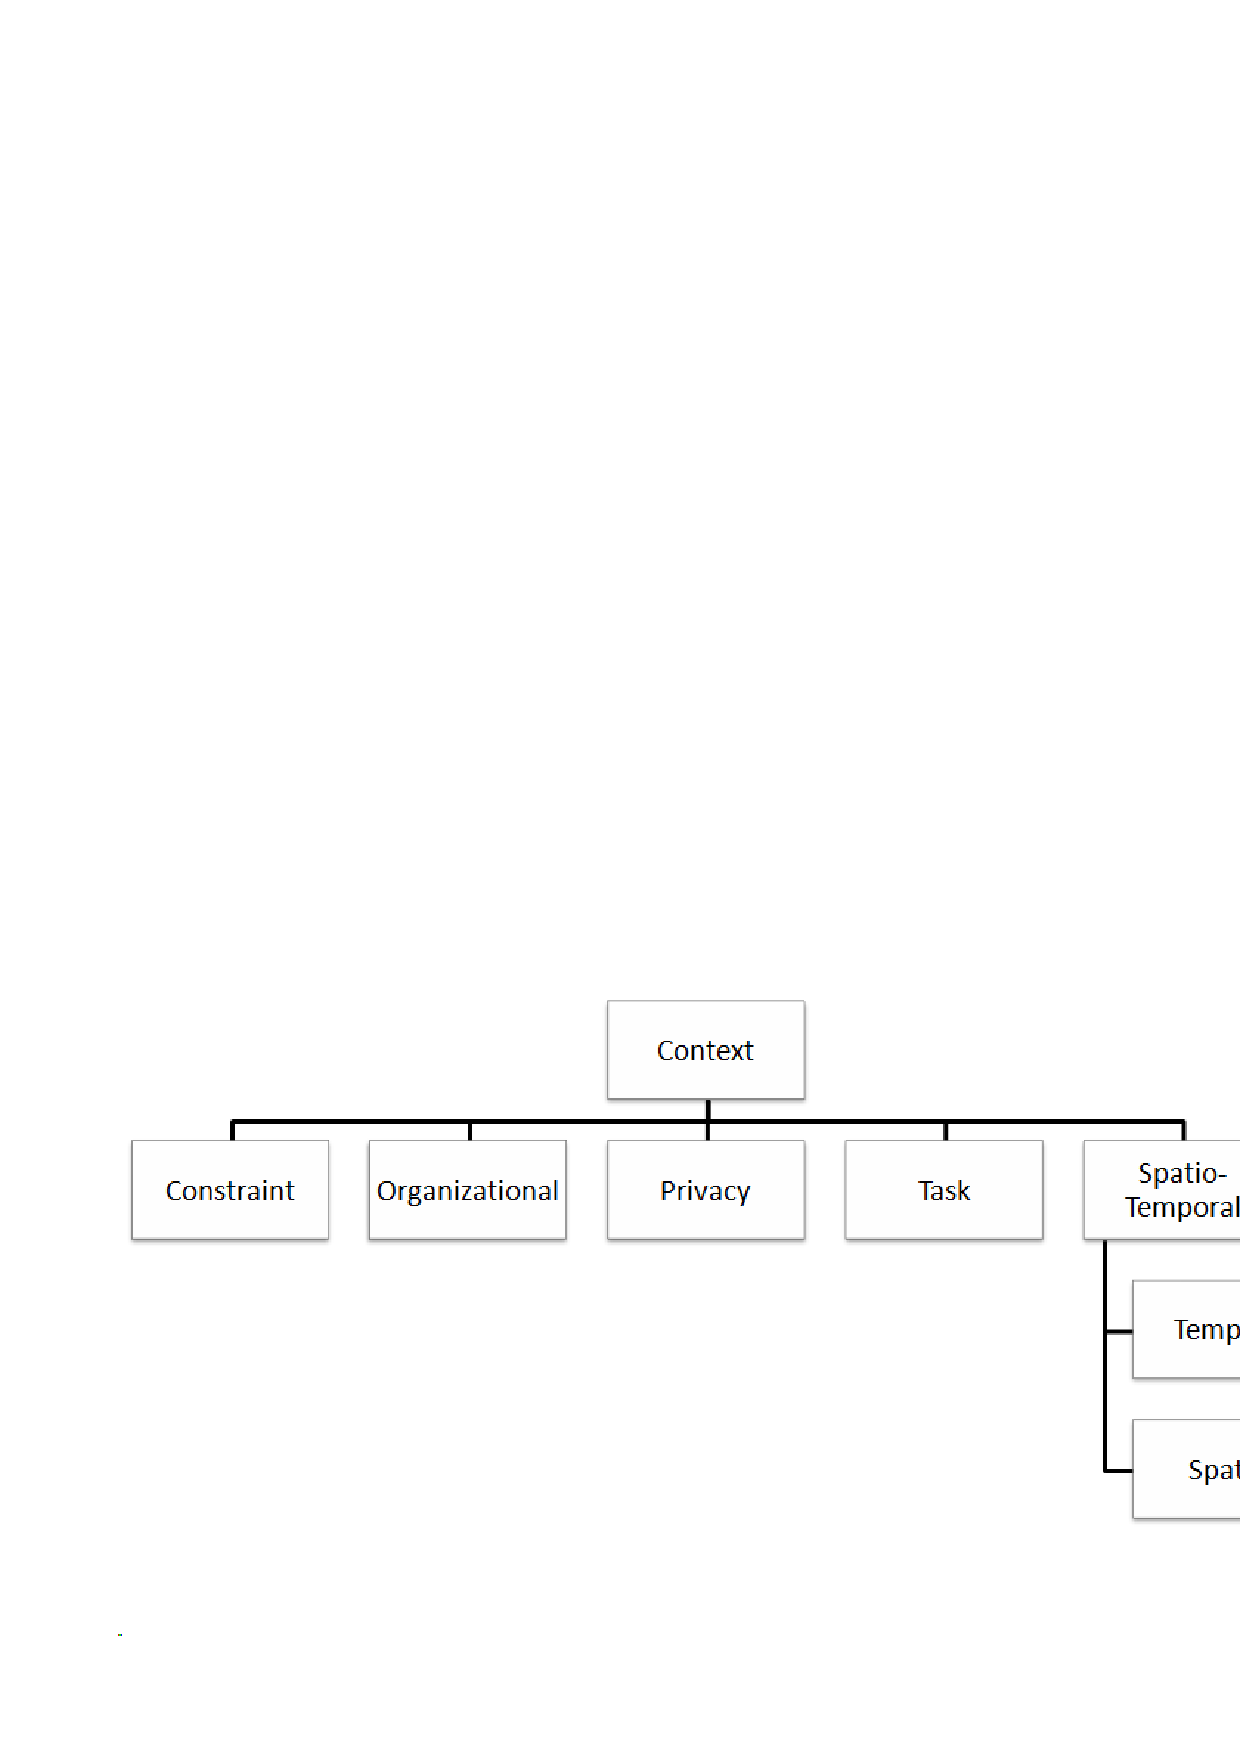
\includegraphics[width=6.0in]{sections/category_structrure.png}
%\vspace{-0.2 in}
    \caption{\label{fig:category_structrure}Structure of categories within the RBAC extension models.}
\end{figure}

\subsection{Analysis and Discussion}

The 27 primary sources produced a set of eight hierarchical categories. 
Table \ref{tab:categorization} summarizes each primary source under their designated category and furthermore, displays the perceived hierarchy of the categories. 
Figure~\ref{fig:category_structrure} shows the hierarchy structure among categories and the counts of primary sources for each.
For categories that have sub-categories, the totals of the category and sub-categories is provided as the second number in the figure. 
The Constraint, Organizational, Privacy, Task, and Spatial and Temporal categories can be special cases of the Context category. 
The Spatial and Temporal categories were treated as subsets of the broader category of Spatio-Temporal since this category encompasses them individually and the Spatio-Temporal category was derived from primary sources directly.

When looking across all categories, we noted that each category added specific features on top of the RBAC Reference Model.
These features were under the surface adding contextual relationships between the core user, permission and role entities. 
Thus, we concluded that all categories stemmed from the context category, of which some primary sources were already deemed direct members.  

For example, in the case of the Privacy category, the models added entities such as purpose binding to represent within the model data collected for one purpose should not be used for another purpose without user consent {\cite{ni2010privacy}. 
While the new entity provided by the Privacy based models is inspired by domains such as healthcare where privacy is of legal concern, the underlying mechanism that drives purpose binding is providing context around making an access control decision. 
The system must take into account not just a static set of permissions a user has through their roles, but also the context of the data being accessed as that data relates to privacy policy. 
In the spatio-temporal models, a users location and the time of day are two factors that can be taken into account when activating a role or verifying a permission.  
The concepts of location and time are properties of the user and place specific contexts around the role and permission entities.

\greybox{We found eight categories that exist within the RBAC extension models: Constraint, Context, Organization, Privacy, Task, Spatio-Temporal, Spatial and Temporal. The context category was a superset of all other categories since all categories were found to consider context.}

\section{Motivations} \label{sec:motivations}

RQ2: What are the motivations behind extensions to RBAC?

\subsection{Results}

\begin{itemize}
\setlength{\itemsep}{0.25pt}
\item Core RBAC model needs additional contextual information and constraints to develop fine-grained policies in practice.
\item Core RBAC does not incorporate context. Therefore, RBAC belongs to static access control model, which may not capture changes in environments.
\item Core RBAC does not support for various constraints such as temporal and spatial constraints to design sophisticated policies on demand.
\item Core RBAC does not provide an abstraction to additional user-defined attributes	(e.g., task and team) and their association with existing attributes.
\item Core RBAC has limitation on delegation and role hierarchy. For example, partial inheritance in role hierarchy needs to be developed.  
\item Model needs to incorporate additional contextual information and constraints to develop fine-grained policies in practice.
\item Model needs to incorporate additional attributes such as
task, team, purpose, organizational roles and collaborative activities over existing attributes. Moreover, new association between attributes
are introduced. 
\item Model needs to improve existing features such delegation and role hierarchy to meet fine-grained access control. 
\end{itemize}

\subsection{Analysis and Discussion}

The RBAC standard model provides an abstraction on top of authorization based on user role assignment (UA) and role
permission assignment (PA). Since this simple model may not provide a fine-grained access control for sophisticated
security mechanism, a variety of extended RBAC models have been proposed over the years to meet
security requirements. When administrators design a model, it is important to capture an important abstraction to help the model to be enforced in a system.

The RBAC standard model presents four entities: roles, sessions, users, and permissions, and their relations. While this model is considered fundamental in any RBAC systems, this model can be extended to be applicable for emerging applications such as healthcare and mobile devices. Such extended RBAC models are formally presented to describe its behaviors. In the selected papers, researchers illustrate how an extended model incorporates new element based on the correct RBAC and describe their relations with pre-defined elements in the core RBAC.

We classify motivations behind RBAC extensions to these three categories:

\begin{itemize}
	\item Addition: an extended model incorporates additional elements with regards to context/constraints and their relations with existing elements of the core RBAC. Models in this category does not change the core model. We found OO papers in this category.
	\item Modification: an extended model incorporates modification of existing features in the core RBAC. For example, changes of attribute relations such as role hierarchy is to show modification. For models in this category, changes occur within the core model. We found OO papers in this category.
	\item Combination: an extended model is combination of RBAC and an another access control model, which uses model-specific attributes and their relations such as task, team, purpose, organizational roles. For this combination, new association between attributes of two models should be introduced. Models in this category requires a new association between attributes of different access control models to work together. We found OO papers in this category.
\end{itemize}

\section{Implementations} \label{sec:implementations}

RQ3: Do the extension models have corresponding implementations?

\subsection{Results}

When designing and proposing a model targeted at a feature that is rooted in practical
usage by real software systems, bringing the model to life is strong evidence that the
proposed model can work in practice. The concept of authorization, and access control
is rooted in a business need. Thus, any access control model needs to be feasible
in the real world not just on paper. We analyzed the primary sources to see how many
proposed models actually had implementations associated with them.  And quantified the
type of implementation. Whether the implementation was for a real system, for a prototype
and/or used in a production environment.

\begin{table}
\centering
\caption{Implementation types found and the count of primary sources}
\begin{tabular}{ | c | c | }
\cline{1-2}

\textbf{Implementation Type} & \textbf{Paper Count} \\ \cline{1-2}
Enterprise Implementation & 4 \\ \cline{1-2}
Prototype Implementation & 4 \\ \cline{1-2}
No Implementation & 20 \\

\cline{1-2}
\end{tabular}
\label{tab:implementations}
\end{table}

Table \ref{tab:implementations} shows the breakdown of implementations found within the primary sources.
Of the 28 papers surveyed, there was a lack of implementation with 20 of the paper providing no
mention of a implementation or prototype.  Of the remaining 8 papers that did mention an implementation, half 
were simply prototypes developed by the authors while the other half were claimed to be implemented within a real
system.

\subsection{Analysis and Discussion}

The RBAC standard was designed with enterprises in mind such that when practitioners implemented RBAC into their systems
there would be a reasonable assurance being based off a well thought out model.  As extensions to the standard model
come along, thought and time should be given to how features and nuances of their models may impact implementation
in order to achieve the same goals as the original standard.  The primary sources should a significant lack of implementation
with over 70\% of the models having no notion of attempting to implement them.  The bare minimum, as 4 papers did, should be
a prototype implementation of the model for review by both practitioners and researchers. Of the models that produced an 
implementation within the enterprise world, two were from within the medical domain and two were implemented using web application technologies.  

\section{Evaluations} \label{sec:evaluations}

RQ4: How are extension to RBAC evaluated theoretically and in practice?

\subsection{Results}

The 28 primary sources were examined for evidence that evaluations of the proposed model were presented by the model authors.
Further, we identified a set of evaluation types found within the each of the primary sources and provide below a list of the 
evaluation types and which primary sources provided which type.  In some cases a single primary source provided multiple evaluation
types.

\begin{itemize}
\setlength{\itemsep}{0.25pt}
\item Time-based Performance \cite{ni2010privacy}, \cite{aich09:role}
\item Complexity analysis \cite{bao08:role}, \cite{zhang06:collaborative}, \cite{chen08:spatio-temporal}, \cite{aich09:role}
\item Comparison to standard RBAC \cite{bao08:role}, \cite{zou2009crbac}, \cite{zhang06:collaborative}, \cite{zhao2008flexible}, \cite{ray07:spatio}
\item Mathematical modeling \cite{damian2007geo}, \cite{hansen2003spatial}, \cite{aich07:STARBAC}, \cite{chen08:spatio-temporal}, \cite{joshi05:generalized}
\item Example scenarios of the model in action \cite{alam06:constraint}, \cite{tzelepi01:flexible}, \cite{cholewka00:acontext-sensitive}, \cite{huang06:pervasive}, \cite{bao08:role}, \cite{jian2008extended}, \cite{yamazaki104:designing}, \cite{zou2009crbac}, \cite{ray07:spatio}, \cite{samuel07:spatio-temporal}, \cite{ray07:spatio}, \cite{joshi05:generalized}, \cite{yao2008task}, \cite{zhou2007team}, \cite{oh2003task}
\item Experimental analysis of the model
\item Case study of the model in practice \cite{motta03:contextual}
\end{itemize}

Based on the diverse evaluation criteria, 12 models presented no evidence of an evaluation. Eight models presented example scenarios
and how application of their model would apply and resolve the situation.  Six of the models provided some form of performance
or complexity analysis of their model.  This included graphs of the model's time to determine authorization as the number of entities
grew, and the size of the role space for the extension model compared to standard RBAC. Four models provided mathematical descriptions
and analysis as a way to provide evaluation in the form of completeness. 
The most widely used evaluation method was providing sample scenarios with accompanying workflows of how the extension model
would tackle those scenarios. Much is left to the reader to assume of these types of evaluations, as the authors do not explicitly state
or show how the standard model is deficient in tackling said scenarios.

\subsection{Analysis and Discussion}

When proposing an access control model, providing an evaluation of the model is a key component in establishing the validity of the model. 
Further, in the case of extensions to the RBAC standard model, the model should be accompanied by validation of the model as a stand-alone
access control model and in comparison to the model upon which the enhancements are being made. The results show that robust evaluations of
extension models are lacking. 

The primary source of validation a developer or practitioner may encounter is a qualitative discussion of real-world
scenarios and how the proposed model can tackle those situations. In rare cases, five primary sources, the model 
authors provide some discussion of how the RBAC standard model is deficient in tackling the scenario. In rarer cases, 
one paper from our results, a case study is performed to examine how the proposed model works in practice. Discussions
of how an extension model handles a real-world scenario provides developers and practitioners anecdotal evidence at best
for what types of situations the proposed model could handle. Further, by not providing a comparison to the RBAC standard
model, developers may be left implementing a more complex model to address their requirements when the standard model would
have sufficed.  Further, given the nature of access control models as grounded in application to enterprise implementations, 
case studies of a model in action provide developers with evidence that the model works as intended when applied.

When looking for an enterprise ready access control mechanism, developers must balance usability with security. 
Two of the primary sources examined provided time-based performance analysis of their extension model compared
to the RBAC standard model. This inclusion of time analysis provides some assurances to developers that any non-functional
requirements surrounding time to compute authorizations compete or beat the standard model. Further, four of the models provided
some form of complexity of their model. This complexity analysis plays a key role in the management of the access control mechanism
over the course of the models implementation lifetime. As the number of roles, users and additional entities grows, developers will 
need to ensure non-functional requirements are met that deal with the ability for a system administrator to effectively manage these
entities.


\section{Domains} \label{sec:domains}

RQ5: What domains have extensions to RBAC been created for?

\subsection{Results}

Business needs have historically driven RBAC research and development.  The primary mode of evaluation for
model extensions has been the presentation of business scenarios in various domains and how the model
uniquely handles those particular scenarios.  Thus, looking for trends in the domains used in the example
scenarios might serve to illuminate a trend worth further examination into the reason for the explosion of
RBAC extensions.  The authors identified domains presented within the primary sources by looking for example
scenarios cast within a particular domain or mention of domain requirements within the body of the paper.
We found that the domains mentioned and their associated sources are:

\begin{itemize}
\setlength{\itemsep}{0.25pt}
\item Medical domain \cite{alam06:constraint}, \cite{tzelepi01:flexible}, \cite{motta03:contextual}, \cite{ni2010privacy}, \cite{damiani2007geo}, \cite{hansen2003spatial}, \cite{samuel07:spatio-temporal}, \cite{aich09:role}, \cite{zhou2007team}
\item Pervasive computing environments \cite{huang06:pervasive}, \cite{chen08:spatio-temporal}, \cite{ray07:spatio}
\item Web applications \cite{masoumzadeh2008purbac}
\item Mobile computing \cite{thein2011leveraging}, \cite{zou2009crbac}, \cite{chandran05:llt}, \cite{ray07:spatio}, \cite{aich09:role}
\item Large-scale organizations with many sub-departments \cite{yamazaki04:designing}, \cite{han08:extended}, \cite{yao2008task}
\item Enterprise, organization workflows \cite{cholewka00:acontext-sensitive}, \cite{bao08:role}, \cite{zhang06:collaborative}, \cite{oh2003task}, \cite{joshi05:generalized}
\end{itemize}

The predominant domain for which extension models have been generated for is that of the medical domain with 9 of 28 mentioning scenarios or requirements of that industry.
Mobile computing and enterprise workflows were each represented by 5 papers claiming to be influenced by the requirements for access control within these domains. The final set
of domains was pervasive computing environments and large-scale organizations with 3 each and web applications with 1.  There were 4 papers without any direct mention of a domain
since Aich et al. \cite{aich09:role} fall under both the medical domain and mobile computing.

\subsection{Analysis and Discussion}

The medical domain produced the largest selection of papers when analyzing the domains influencing the proposals of extension models.  
Further, the authors noted that the categories associated with papers identifying the medical domain was not limited to one or two but cut across
each of the eight categories except for Organization. 
The cross-category nature of the medical domain papers appears indicative of the complex nature of medical applications and the requirements therein.
Given the growth of the research and development of medical applications over the past decade this result does not appear to be surprising. However,
the RBAC standard was originally created to reduce cost and increase interoperability - two goals of current regulation around the standardization
of electronic health record systems. The large number of proposed models, and the cross-category result stand in direct opposition of the goals
of both the RBAC standard and current regulations.

The RBAC standard has been re-enforced by the economic impact that standardization has had on enterprises needing to apply access control.  The
inclusion of extension models targeted at the enterprise workflow domain is indicative of the expansion of requirements for enterprises. Developers
and researchers should take care when looking at extension models designed to addresses the newer requirements of enterprise workflows in order to
achieve the same economic implementation and maintainability benefits the original standard model presents.

Mobile computing has seen a dramatic increase in the number of available devices, operating systems and applications since 1997 when the first smart phone
was introduced. 
The domain analysis results produced five papers that targeted extensions that are designed to address the requirements of mobile computing.
For a domain that has roots in personal and enterprise computing, protecting the data of both through access controls is paramount given their ubiquity.


\section{Generaliations} \label{sec:generalizations}

RQ6: What commonalities or generalizations exist across all categories?

\subsection{Results}

Core or any extended role-based access control is used in various aspects of computer systems. In order to reduce efforts for modeling access control used in various applications, researchers often focus on developing generalized core concepts of access control.
We found that propositional logic is used to describe access control model across all categorizations. Propositional logic is concerned with propositions and their logical relationships. In propositional logic, simple (i.e., atomic) or compound condition at given context is evaluated to true or false based on specified rules and access control logic. Researchers are concerned to extend limited set of propositions specific to core RBAC to meet real-world scenarios such as dynamic constraints, temporal, or spatial constraints. However, semantic meanings of such propositions are various based on researchers' intention.

\subsection{Analysis and Discussion}

Since NIST proposed RBAC standard using propositional logic, researchers describe extended RBAC models using propositional logic. Given context, propositional logic is used to evaluate true or false based on specified rules and access control logic. As access control is typically evaluated to either true (Permit) or false (Deny) based on predicates, propositional logic is sufficient to describe key ideas and definitions. We found that OO papers of RBAC extensions use propositional logic to describe its extended model.
However, propositional logic has limitations. While this logic is simple, this logic does not support for reasoning about RBAC, which helps reduce the administrative complexity of associations such as user- role associations. An alternative logic to describe RBAC is first-order logic. This logic is sufficient to describe RBAC and extended RBAC. Moreover, this logic supports for concise and elegant formulation of the RBAC model and its relation.  First-Order logic is expressive enough to concisely represent access control systems. First-Order logic uses relations, variables, and quantifiers.

\section{Conclusion} \label{sec:conclusion}

The RBAC extension models were revealed to fall into a number of categorizations with Organization, Privacy, Resource, Task, Spatio-Temporal, Spatial, and Temporal falling under the general category of context.
The categories each had properties specific to their implementation, but were seen to generalize to being specialized instances of context tailored to the entities or actions the categories covered.
A number of domains were identified as being the motivations behind needing extensions to the RBAC Reference model.  The domains, such as healthcare, presenting new challenges the previous models were not
required to design for.  Our literature review showed that the state of RBAC extension model evaluation needs focused from the research community given most model evaluations seen within the papers were
based on hypothetical situations with little to no case studies or implementations in practice.



%% REFERENCES %%
\bibliographystyle{elsarticle-num}
\bibliography{sections/rbacslr}

%% Outline - REMOVE ME %%
\section{Outline}

\begin{enumerate}
\item Introduction
    \begin{itemize}
  	\item RBAC history, RBAC as a standard
  	\item Audience that should care about our review
  	\item Brief explanation of what has led to extensions cropping up
	  	\item Paper organization
    \end{itemize}
\item Background
    \begin{itemize}
   	\item What is RBAC
   	\item Core RBAC and it's entities, and what it tries to solve
    \end{itemize}
\item Process
\item Results
    \begin{itemize}
  	\item Data used in process, results of process for paper count
  	\item Categorization that came out applying process (based on word usage)
  	\item Results for each research question (raw data)
    \end{itemize}
\item Analysis
    \begin{itemize}
  	\item Explanation and definitions of categories based on results
  	\item Examination of results in relation to each research question and larger trends drawn from data
  	\item Examination of cross research question concerns an
    \end{itemize}
\item Conclusion
\end{enumerate}

\section{Appendix} \label{sec:appendix}

\begin{table}
\centering
\begin{tabular}{|p{12.5cm}|p{3cm}|}
\hline
\textbf{Paper} & \textbf{Category}
\\\hline
A constraint based role based access control in the SECTET a model-driven approach, 2006 \cite{alam06:constraint} & Constraint \\\hline

A flexible content and context-based access control model for multimedia medical image database systems, 2001 \cite{tzelepi01:flexible} & Context \\\hline

A context-sensitive access control model and prototype implementation, 2000 \cite{cholewka00:acontext-sensitive} & Context \\\hline

A Context, Rule and Role-Based Access Control Model In Enterprise Pervasive Computing Environment, 2006 \cite{huang06:pervasive} & Context \\\hline

A contextual role-based access control authorization model for electronic patient record Motta, 2003 \cite{motta03:contextual} & Context \\\hline

A Role and Context Based Access Control Model with UML, 2008 \cite{bao08:role} & Context \\\hline

An extended RBAC model based on granular logic, 2008 \cite{jian2008extended} & Context \\\hline

Designing an agent-based RBAC system for dynamic security policy, 2004 \cite{yamazaki104:designing} & Context \\\hline

An extended RBAC model based on granular logic, 2008 \cite{han08:extended} & Context \\\hline

Leveraging Access Control Mechanism of Android Smartphone Using Context-Related Role-Based Access Control Model, 2011 \cite{thein2011leveraging} & Context \\\hline

CRBAC: Imposing multi-grained constraints on the RBAC model in the multi-application environment, 2009 \cite{zou2009crbac} & Context \\\hline

ROBAC: Scalable Role and Organization Based Access Control Models, 2006 \cite{zhang06:collaborative} & Organizational \\\hline

Privacy-aware role-based access control, 2007 \cite{ni2010privacy} & Privacy \\\hline

PuRBAC: Purpose-Aware Role-Based Access Control, 2008 \cite{masoumzadeh2008purbac} & Privacy \\\hline

A Flexible Role- and Resource-Based Access Control Model, 2008 \cite{zhao2008flexible} & Resource \\\hline

GEO-RBAC: a spatially aware RBAC, 2005 \cite{damian2007geo} & Spatial \\\hline

LRBAC: A location-aware role-based access control model, 2006 \cite{ray07:spatio} & Spatial \\\hline

Spatial role-based access control model for wireless networks, 2003 \cite{hansen2003spatial} & Spatial \\\hline

STARBAC: Spatiotemporal role based access control, 2007 \cite{aich07:STARBAC} & Spatio-Temporal \\\hline

On spatio-temporal constraints and inheritance in role-based access control, 2008 \cite{chen08:spatio-temporal} & Spatio-Temporal \\\hline

A framework for specification and verification of generalized spatio-temporal role based access control model, 2007 \cite{samuel07:spatio-temporal} & Spatio-Temporal \\\hline

LoT-RBAC: A Location and Time-Based RBAC Model, 2005 \cite{chandran05:llt} & Spatio-Temporal \\\hline

A Spatio-temporal Role-Based Access Control Model, 2007 \cite{ray07:spatio} & Spatio-Temporal \\\hline

Role Based Access Control with Spatiotemporal Context for Mobile Applications, 2009 \cite{aich09:role} & Spatio-Temporal \\\hline

A Task-Role Based Access Control Model with Multi-Constraints, 2008 \cite{yao2008task} & Task \\\hline

Team and Task Based RBAC Access Control Model, 2009 \cite{zhou2007team} & Task \\\hline

Task-role-based access control model, 2003 \cite{oh2003task} & Task \\\hline

A generalized temporal role-based access control model, 2005 \cite{joshi05:generalized} & Temporal \\\hline

\end{tabular}
\caption{Primary sources grouped by categorization}
\label{tab:categorization}
\end{table}


\end{document}
